% This is samplepaper.tex, a sample chapter demonstrating the
% LLNCS macro package for Springer Computer Science proceedings;
% Version 2.20 of 2017/10/04
%
\documentclass[runningheads]{llncs}
%
\usepackage{graphicx}
\usepackage{ctex}
\usepackage{xeCJK}
% Used for displaying a sample figure. If possible, figure files should
% be included in EPS format.
%
% If you use the hyperref package, please uncomment the following line
% to display URLs in blue roman font according to Springer's eBook style:
% \renewcommand\UrlFont{\color{blue}\rmfamily}

\begin{document}
%
\title{LGLT:Line graph linear-complexity transformer for 3d skeleton-based action recognition\thanks{Supported by organization x.}}
%
%\titlerunning{Abbreviated paper title}
% If the paper title is too long for the running head, you can set
% an abbreviated paper title here
%
\author{First Author\inst{1}\orcidID{0000-1111-2222-3333} \and
Second Author\inst{2,3}\orcidID{1111-2222-3333-4444} \and
Third Author\inst{3}\orcidID{2222--3333-4444-5555}}
%
\authorrunning{F. Author et al.}
% First names are abbreviated in the running head.
% If there are more than two authors, 'et al.' is used.
%
\institute{Princeton University, Princeton NJ 08544, USA \and
Springer Heidelberg, Tiergartenstr. 17, 69121 Heidelberg, Germany
\email{lncs@springer.com}\\
\url{http://www.springer.com/gp/computer-science/lncs} \and
ABC Institute, Rupert-Karls-University Heidelberg, Heidelberg, Germany\\
\email{\{abc,lncs\}@uni-heidelberg.de}}
%
\maketitle              % typeset the header of the contribution
%
\begin{abstract}
The abstract should briefly summarize the contents of the paper in
15--250 words.

\keywords{First keyword  \and Second keyword \and Another keyword.}
\end{abstract}
%
%
%
\section{Introduction}
\subsection{A Subsection Sample}

Skeleton-based action recognition has emerged as a critical research 
direction in computer vision, driven by its applications in healthcare 
monitoring \cite{ref1}, human-computer interaction \cite{ref2}, and surveillance systems \cite{ref3}.
Early approaches primarily relied on Recurrent Neural Networks (RNNs) \cite{ref4,ref5} 
to model temporal dependencies and Convolutional Neural Networks (CNNs) \cite{ref6}
to process joint coordinates as pseudo-images. While these methods achieved 
reasonable performance, they struggled to capture the intrinsic spatial 
relationships between joints, particularly for fine-grained actions 
requiring nuanced motion analysis \cite{ref7}.


The advent of Graph Convolutional Networks (GCNs) \cite{ref8} revolutionized the field by 
explicitly modeling skeletal topology through adjacency matrices. Pioneering 
work like ST-GCN \cite{ref7} introduced spatial-temporal convolutions to jointly 
capture joint correlations across frames. Subsequent innovations proposed 
learnable adjacency matrices \cite{ref9,ref10} and multi-scale aggregation 
strategies \cite{ref11} to enhance flexibility.Despite these advancements, 
two critical limitations persist:

Subsequent paragraphs, however, are indented.

一些中文字符。

\subsubsection{Sample Heading (Third Level)} Only two levels of
headings should be numbered. Lower level headings remain unnumbered;
they are formatted as run-in headings.

\paragraph{Sample Heading (Fourth Level)}
The contribution should contain no more than four levels of
headings. Table~\ref{tab1} gives a summary of all heading levels.

\begin{table}
\caption{Table captions should be placed above the
tables.}\label{tab1}
\begin{tabular}{|l|l|l|}
\hline
Heading level &  Example & Font size and style\\
\hline
Title (centered) &  {\Large\bfseries Lecture Notes} & 14 point, bold\\
1st-level heading &  {\large\bfseries 1 Introduction} & 12 point, bold\\
2nd-level heading & {\bfseries 2.1 Printing Area} & 10 point, bold\\
3rd-level heading & {\bfseries Run-in Heading in Bold.} Text follows & 10 point, bold\\
4th-level heading & {\itshape Lowest Level Heading.} Text follows & 10 point, italic\\
\hline
\end{tabular}
\end{table}


\noindent Displayed equations are centered and set on a separate
line.
\begin{equation}
x + y = z
\end{equation}
Please try to avoid rasterized images for line-art diagrams and
schemas. Whenever possible, use vector graphics instead (see
Fig.~\ref{fig1}).

\begin{figure}
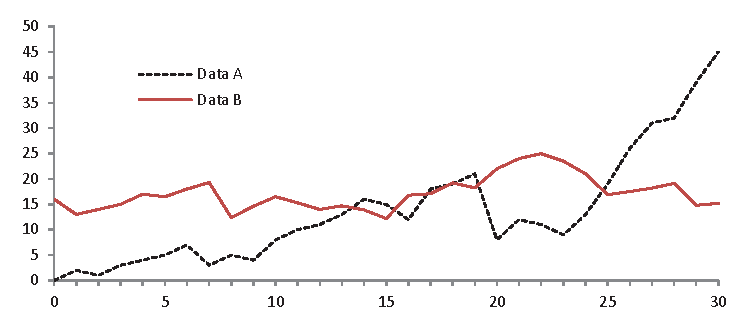
\includegraphics[width=\textwidth]{fig1.eps}
\caption{A figure caption is always placed below the illustration.
Please note that short captions are centered, while long ones are
justified by the macro package automatically.} \label{fig1}
\end{figure}

\begin{theorem}
This is a sample theorem. The run-in heading is set in bold, while
the following text appears in italics. Definitions, lemmas,
propositions, and corollaries are styled the same way.
\end{theorem}
%
% the environments 'definition', 'lemma', 'proposition', 'corollary',
% 'remark', and 'example' are defined in the LLNCS documentclass as well.
%
\begin{proof}
Proofs, examples, and remarks have the initial word in italics,
while the following text appears in normal font.
\end{proof}
For citations of references, we prefer the use of square brackets
and consecutive numbers. Citations using labels or the author/year
convention are also acceptable. The following bibliography provides
a sample reference list with entries for journal
articles~\cite{ref_article1}, an LNCS chapter~\cite{ref_lncs1}, a
book~\cite{ref_book1}, proceedings without editors~\cite{ref_proc1},
and a homepage~\cite{ref_url1}. Multiple citations are grouped
\cite{ref_article1,ref_lncs1,ref_book1},
\cite{ref_article1,ref_book1,ref_proc1,ref_url1}.
%
% ---- Bibliography ----
%
% BibTeX users should specify bibliography style 'splncs04'.
% References will then be sorted and formatted in the correct style.
%
% \bibliographystyle{splncs04}
% \bibliography{mybibliography}
%
% \begin{thebibliography}{8}


% \bibitem{ref1}
% Shahroudy A, Liu J, et al.: NTU RGB+D: A Large Scale Dataset for 3D Human Activity Analysis
% .  Proceedings of the IEEE conference on computer vision and pattern recognition(CVPR) 2016, pp. 1010–1019.

% \bibitem{ref2}
% Liu J, Shahroudy A, et al.: NTU RGB+D 120: A Large-Scale Benchmark for 3D Human Activity Understanding
% , IEEE Trans. Pattern Anal. Mach. Intell. \textbf{42}(10), 2684–2701 (2020)



% \bibitem{ref3}
% Shao D, Zhao Y, et al.:FineGym: A Hierarchical Video Dataset for Fine-grained Action Understanding.  Proceedings of the IEEE conference on computer vision and pattern recognition(CVPR) 2020, pp. 2616-2625.

% \bibitem{ref4}
% Du Y, Wang W, et al.:Hierarchical Recurrent Neural Network for Skeleton-Based Action Recognition.
% Proceedings of the IEEE conference on computer vision and pattern recognition(CVPR) 2015, pp. 1110-1118.

% \bibitem{ref5}
% Du Y, Wang W, et al.:An End-to-End Spatio-Temporal Attention Model for Human Action Recognition
% from Skeleton Data.
% Proceedings of the AAAI conference on artificial intelligence(AAAI), 2017, Vol. 31. No. 1.


% \bibitem{ref6}
% Ke Q, Bennamoun M, et al.:A New Representation of Skeleton Sequences for 3D Action Recognition.
% Proceedings of the IEEE conference on computer vision and pattern recognition(CVPR) 2017, pp. 3288-3297.

% \bibitem{ref7}
% Yan S, Xiong Y,et al.:Spatial Temporal Graph Convolutional Networks for Skeleton-Based Action Recognition.
% Proceedings of the AAAI conference on artificial intelligence(AAAI), 2018, Vol. 32. No. 1.

% \bibitem{ref8}
% Kipf T N, Welling M.:Semi-supervised classification with graph convolutional networks.2016, arXiv:1609.02907.
% \bibitem{ref9}
% Liu Z, Zhang H,et al.:Disentangling and Unifying Graph Convolutions for SkeletonBased Action Recognition.
% Proceedings of the IEEE conference on computer vision and pattern recognition(CVPR) 2020, pp.143-152.

% \bibitem{ref10}
% Chen Y, Zhang Z,et al. :Channel-Wise Topology Refinement Graph Convolution.
% Proceedings of the IEEE conference on computer vision and pattern recognition(CVPR) 2021, pp. 13359-13368.

% \bibitem{ref11}
% Chen Z, Li S,  et al.:Multi-Scale Spatial Temporal Graph Convolutional Network.
% Proceedings of the AAAI conference on artificial intelligence(AAAI), 2018, Vol. 35. No. 2.


% \bibitem{ref_book1}
% Author, F., Author, S., Author, T.: Book title. 2nd edn. Publisher,
% Location (1999)

% \bibitem{ref_proc1}
% Author, A.-B.: Contribution title. In: 9th International Proceedings
% on Proceedings, pp. 1--2. Publisher, Location (2010)

% \bibitem{ref_lncs1}
% Author, F., Author, S.: Title of a proceedings paper. In: Editor,
% F., Editor, S. (eds.) CONFERENCE 2016, LNCS, vol. 9999, pp. 1--13.
% Springer, Heidelberg (2016). \doi{10.10007/1234567890}

% \bibitem{ref_url1}
% LNCS Homepage, \url{http://www.springer.com/lncs}. Last accessed 4
% Oct 2017
% \end{thebibliography}

% 添加 BibTeX 引用指令
\bibliographystyle{splncs04}
\bibliography{references}

\end{document}
